\section{Background}
In a eukaryotic cell, all DNA-templated processes including replication, transcription, and recombination must occur in the context of the local chromatin environment.  The most basic unit of chromatin is the nucleosome, 147 bp of DNA wrapped around an octamer of histones\citep{McGinty2015-kd}.  The dynamic packaging and organization of DNA into chromatin facilitates accessibility of DNA binding factors and is fundamental to regulating gene expression\citep{Kouzarides2007-sk}. Chromatin state has long been correlated with transcription and DNA replication\citep{Stambrook1970-jm,Goldman1984-im}.  For example, gene expression and early DNA replication in S-phase are associated with `active' chromatin states\citep{Rhind2013-yr}. Importantly, because chromatin state is a dynamic feature of the genome, it allows for developmental and cell type specific plasticity in regulating the transcription and DNA replication programs\citep{Goren2008-wr}.  Our research is focused on understanding the mechanisms by which the local chromatin landscape modulates DNA replication, transcription and DNA repair.

The last few years have seen remarkable progress in our understanding of the mechanisms that regulate eukaryotic DNA replication.  A perfect convergence of structural biochemistry\citep{Bleichert2015-zl,Li2015-zi,Yuan2017-gq}, biochemical reconstitution of replication initiation\citep{Yeeles2015-pe,Devbhandari2017-fh,Azmi2017-gg}, and single molecule imaging\citep{Ticau2015-gg} has provided exciting new insights into the initiation of DNA replication and establishment of the replisome.  However, despite the progress made \invitro, our understanding of how individual start sites of DNA replication are selected and regulated in the context of the chromosome to ensure genetic and epigenetic inheritance is poorly understood\citep{Prioleau2016-bj}. \begin{floatingfigure}[lt]{3in}
\vspace{-4mm}
\begin{center}
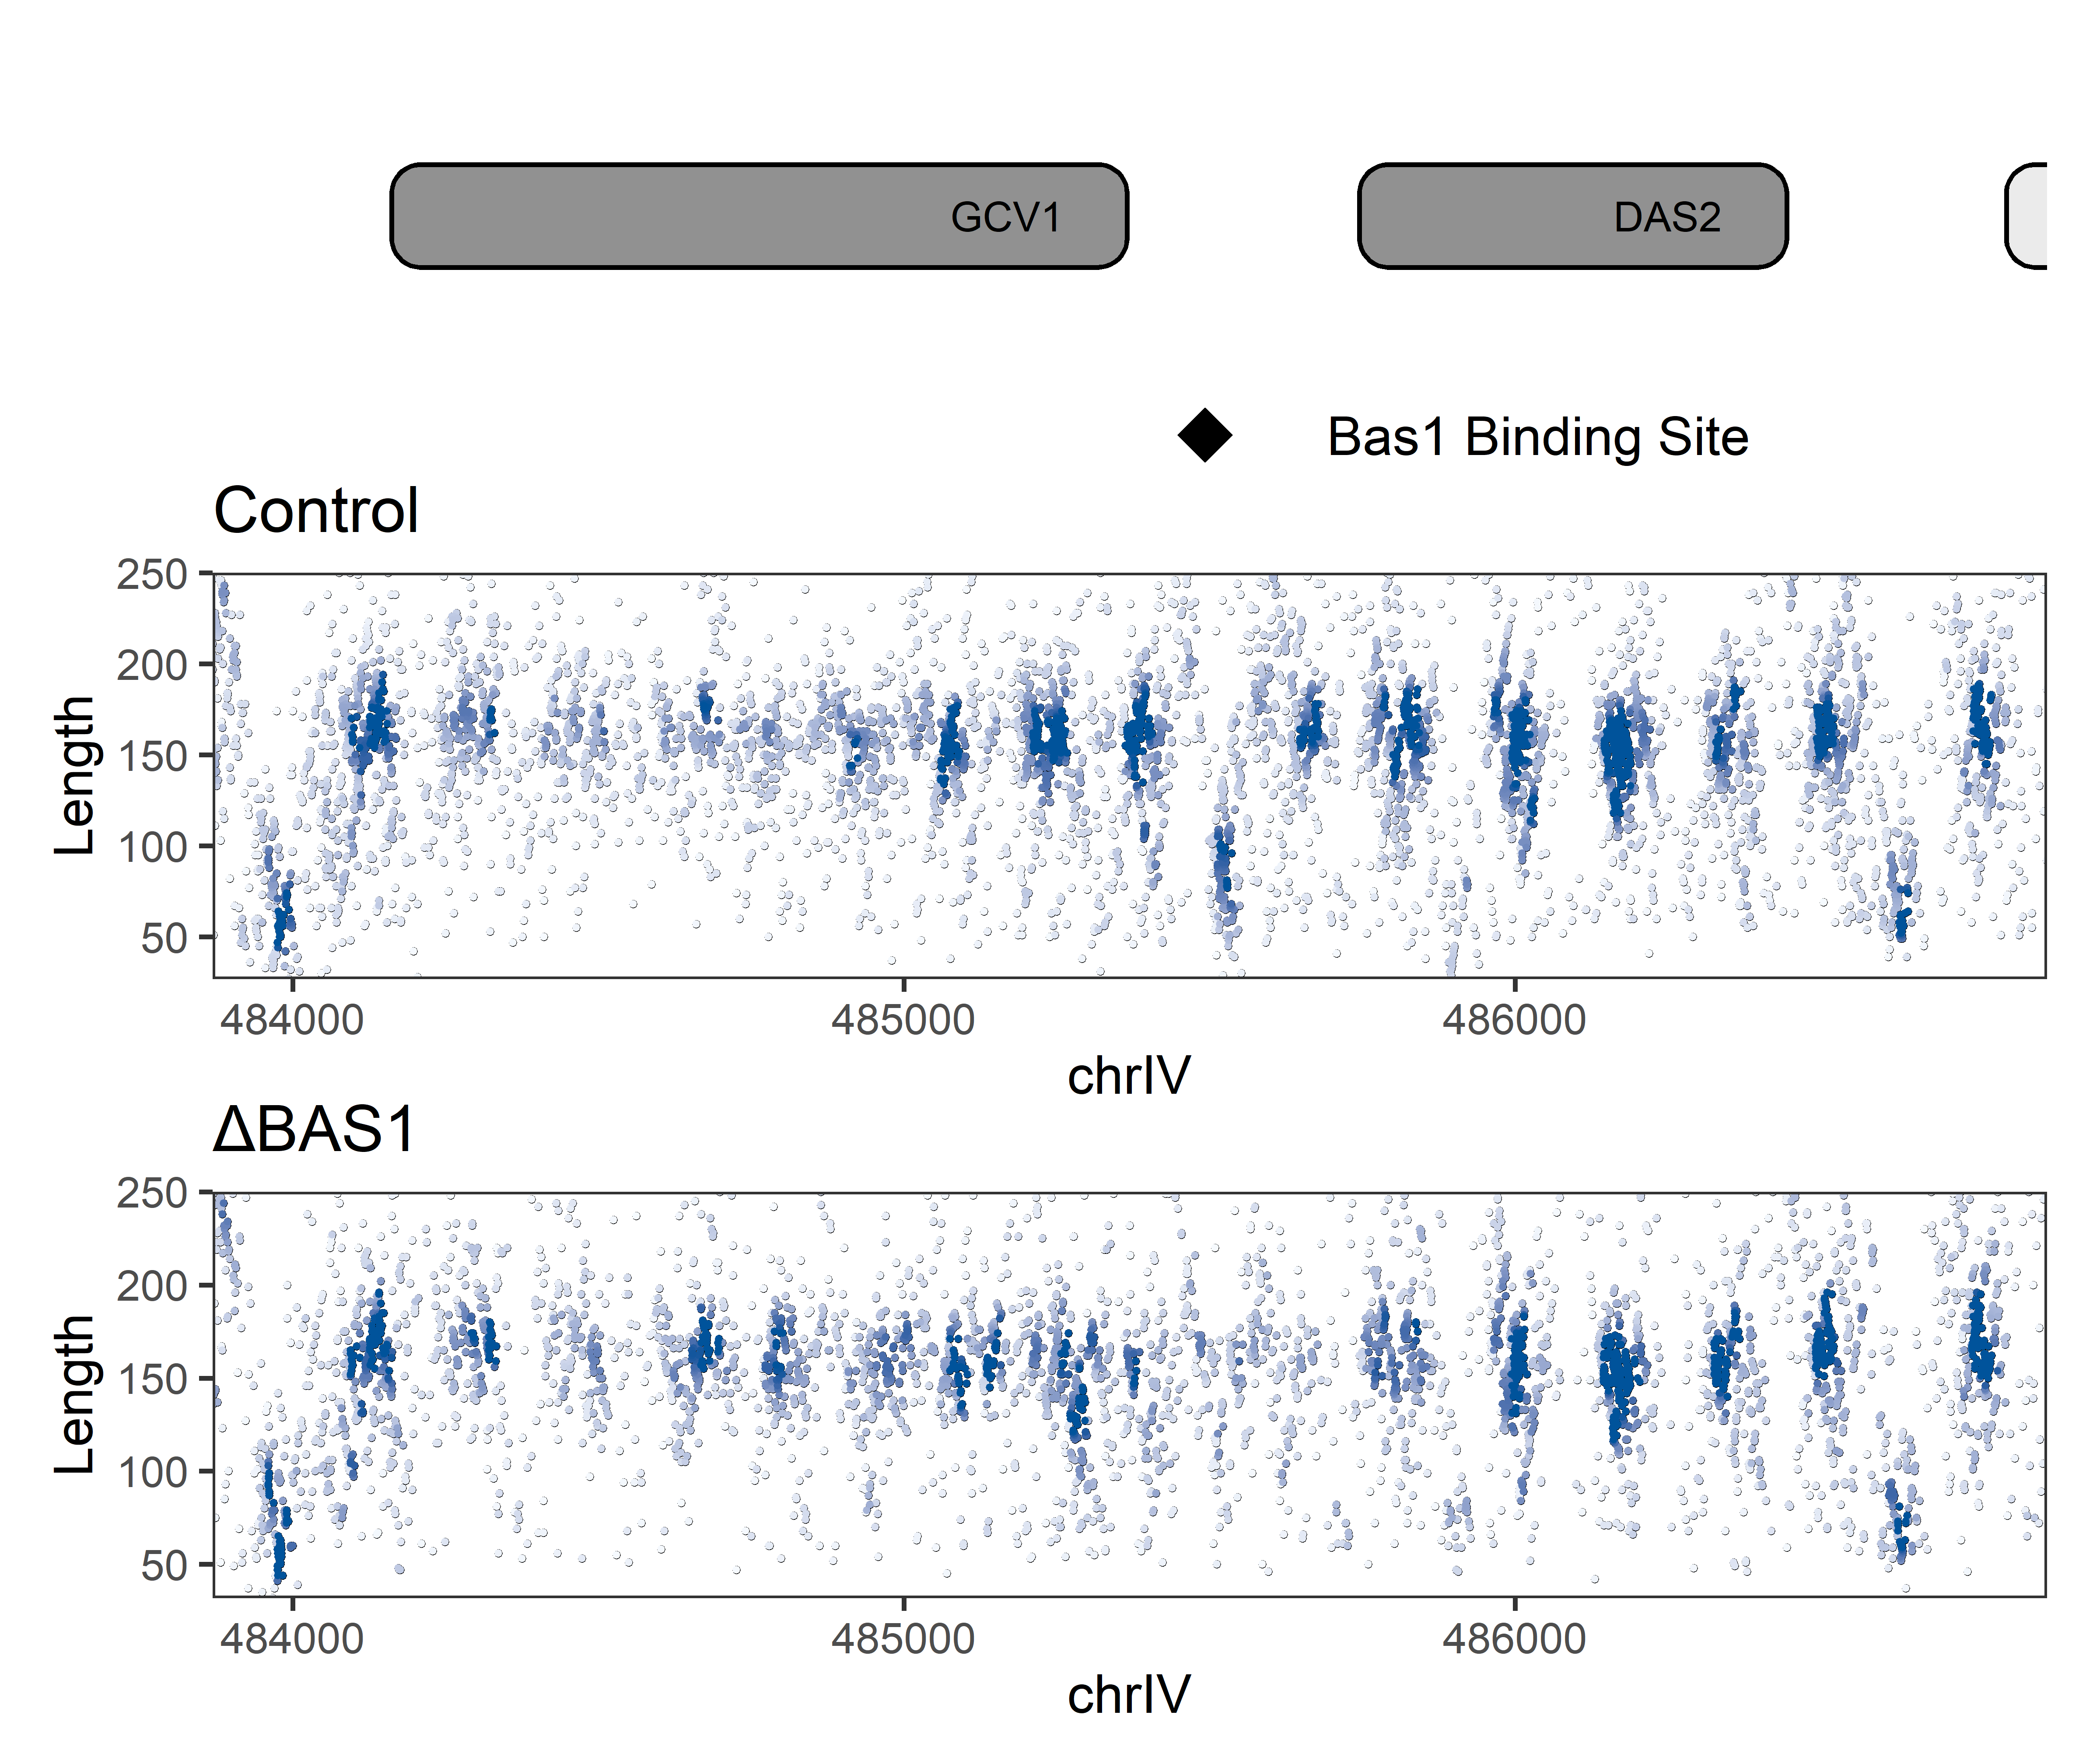
\includegraphics[width=3in]{r35_figures/BAS1_GCV1_typhoon.png}
\end{center}
\vspace{3mm}
\caption{GCOP of a replication origin.  MNase protected DNA fragments were subjected to paired-end sequencing and the resulting fragment lengths were plotted as a function of chromosomal position.  Well phased fragments at $\sim$150 bp represent sequences protected by nucleosomes (red ovals in cartoon) and smaller fragments represent other DNA binding factors (\eg ORC at the ACS and Abf1).  In an \textit{ORC1-161} mutant the footprint at the ACS disappears at the non-permissive temperature.}%
\end{floatingfigure}%

In order to duplicate a chromosome within the confines of S-phase, DNA replication must begin at multiple sites along the chromosome.  Failure to completely replicate the chromosomes may result in catastrophic genomic instability\citep{Green2010-ht}.  Origins of DNA replication are defined by conserved trans-acting factors that assemble on the DNA in  a cell cycle regulated manner. %({\color{dukeblue}\textbf{Figure 1}}). 
The origin recognition complex (ORC) functions together with Cdc6 and Cdt1 to load the Mcm2-7 helicase as a double hexamer and form the pre-replicative complex (pre-RC)\citep{Bell2013-pk}. Pre-RC assembly is limited to G1 and serves to `license' the origin for activation in the subsequent S-phase\citep{Siddiqui2013-jz}. As cells enter S-phase, DDK and CDK promote the recruitment of additional proteins including Cdc45 and the GINS complex to form the pre-initiation complex (pre-IC)\citep{Tanaka2013-fl} ultimately resulting in an active helicase complex at each fork.   

In yeast, DNA replication origins are defined by the ACS (ARS consensus sequence), a cis-acting sequence element that is necessary, but not sufficient, for ORC binding and origin function\citep{Breier2004-tw} suggesting that additional chromatin features modulate origin selection and activation.  In higher eukaryotes ORC exhibits little sequence specificity\citep{Vashee2003-xr} and is preferentially enriched in open and accessible chromatin\citep{MacAlpine2010-ju,Miotto2016-jt}.   We and others have shown that precise nucleosome positioning and active histone exchange are conserved features of ORC binding in yeast\citep{Eaton2010-fq,Berbenetz2010-hh}, \dros\citep{Liu2015-nr,MacAlpine2010-ju} and mammalian cells\citep{Lombrana2013-aw,Lubelsky2011-dj}.  Despite the identification of specific ORC binding sites in mammals\citep{Miotto2016-jt}, the mapping of origins has been challenging and controversial\citep{Prioleau2016-bj}.  Recent Okazaki fragment mapping across the human genome identified only a few sites where initiation could be mapped within 5 kb; instead, the vast majority of initiation events mapped to broad zones of 30 kb or more\citep{Petryk2016-rr}.  If ORC localizes to discrete sites of open chromatin\citep{MacAlpine2010-ju,Miotto2016-jt}, why are initiation events so dispersed?  One intriguing possibility is that the Mcm2-7 complex may not be restricted to ORC proximal sequences following pre-RC assembly and that the location and density of Mcm2-7 complexes may be responsible for the seemingly stochastic origin activation patterns observed in higher eukaryotes. Alternatively, provocative experiments from the Dutta laboratory suggest an ORC-independent mode of Mcm2-7 loading in mammalian cancer cells\citep{Shibata2016-uc}. 

We continue to develop and extend our genome-wide chromatin occupancy profiling (GCOP) assay which provides a factor agnostic near nucleotide resolution view of proteins bound to DNA\citep{}.  Briefly, total chromatin is digested with micrococcal nuclease (MNase) and all of the recovered DNA fragments are subjected to paired-end next-generation sequencing.  The paired-end sequencing of each protected fragment provides two important pieces of data, the location in the genome where the fragment maps to and the size of the fragment.  Importantly, the size of the protected fragment reveals whether it was protected by a nucleosome ($\sim$147 bp) or a DNA-binding factor ($<$50 bp). This assay is factor agnostic and reveals specific footprints for more than 70\% of the yeast DNA-binding factors\citep{Henikoff2011-vo}. The assay only reveals the occupancy state of the DNA; however, we are frequently able to  infer the identify of the bound factor from motifs\citep{} and prior genomic experiments\citep{many}.   

%Our research is focused on understanding the mechanisms by which the local chromatin landscape modulates DNA replication, transcription and the repair of DNA breaks.



%and also the mechanisms by which chromatin structure is re-established in the wake of the replication fork or following repair of broken DNA.  







%Chromatin environment specifies DNA replication
%Replication --> re-establishement of chromatin
%Chromatin and DNA repair 




%However, the likely diverse mechanisms by which the local chromatin environment regulates origin selection and activation at discrete loci remain to determined.

%The last few years have seen remarkable progress in our understanding of the mechanisms that regulate eukaryotic DNA replication.  A perfect convergence of structural biochemistry\citep{Bleichert2015-zl}, biochemical reconstitution of replication initiation\citep{Yeeles2015-pe}, and single molecule imaging\citep{Ticau2015-gg} has provided exciting new mechanistic insights into the initiation of DNA replication and establishment of the replisome.  However, despite the progress made \invitro, our understanding of how individual start sites of DNA replication are selected and regulated in the context of the chromosome to ensure genetic and epigenetic inheritance is poorly understood\citep{Prioleau2016-bj}. 





%The last few years have seen remarkable progress in our understanding of the mechanisms that regulate eukaryotic DNA replication.  A perfect convergence of structural biochemistry\citep{Bleichert2015-zl}, biochemical reconstitution of replication initiation\citep{Yeeles2015-pe}, and single molecule imaging\citep{Ticau2015-gg} has provided exciting new mechanistic insights into the initiation of DNA replication and establishment of the replisome.  However, despite the progress made \invitro, our understanding of how individual start sites of DNA replication are selected and regulated in the context of the chromosome to ensure genetic and epigenetic inheritance is poorly understood\citep{Prioleau2016-bj}. 
%\begin{floatingfigure}[r]{2.5in}
%\vspace{-8mm}
%\begin{center}
%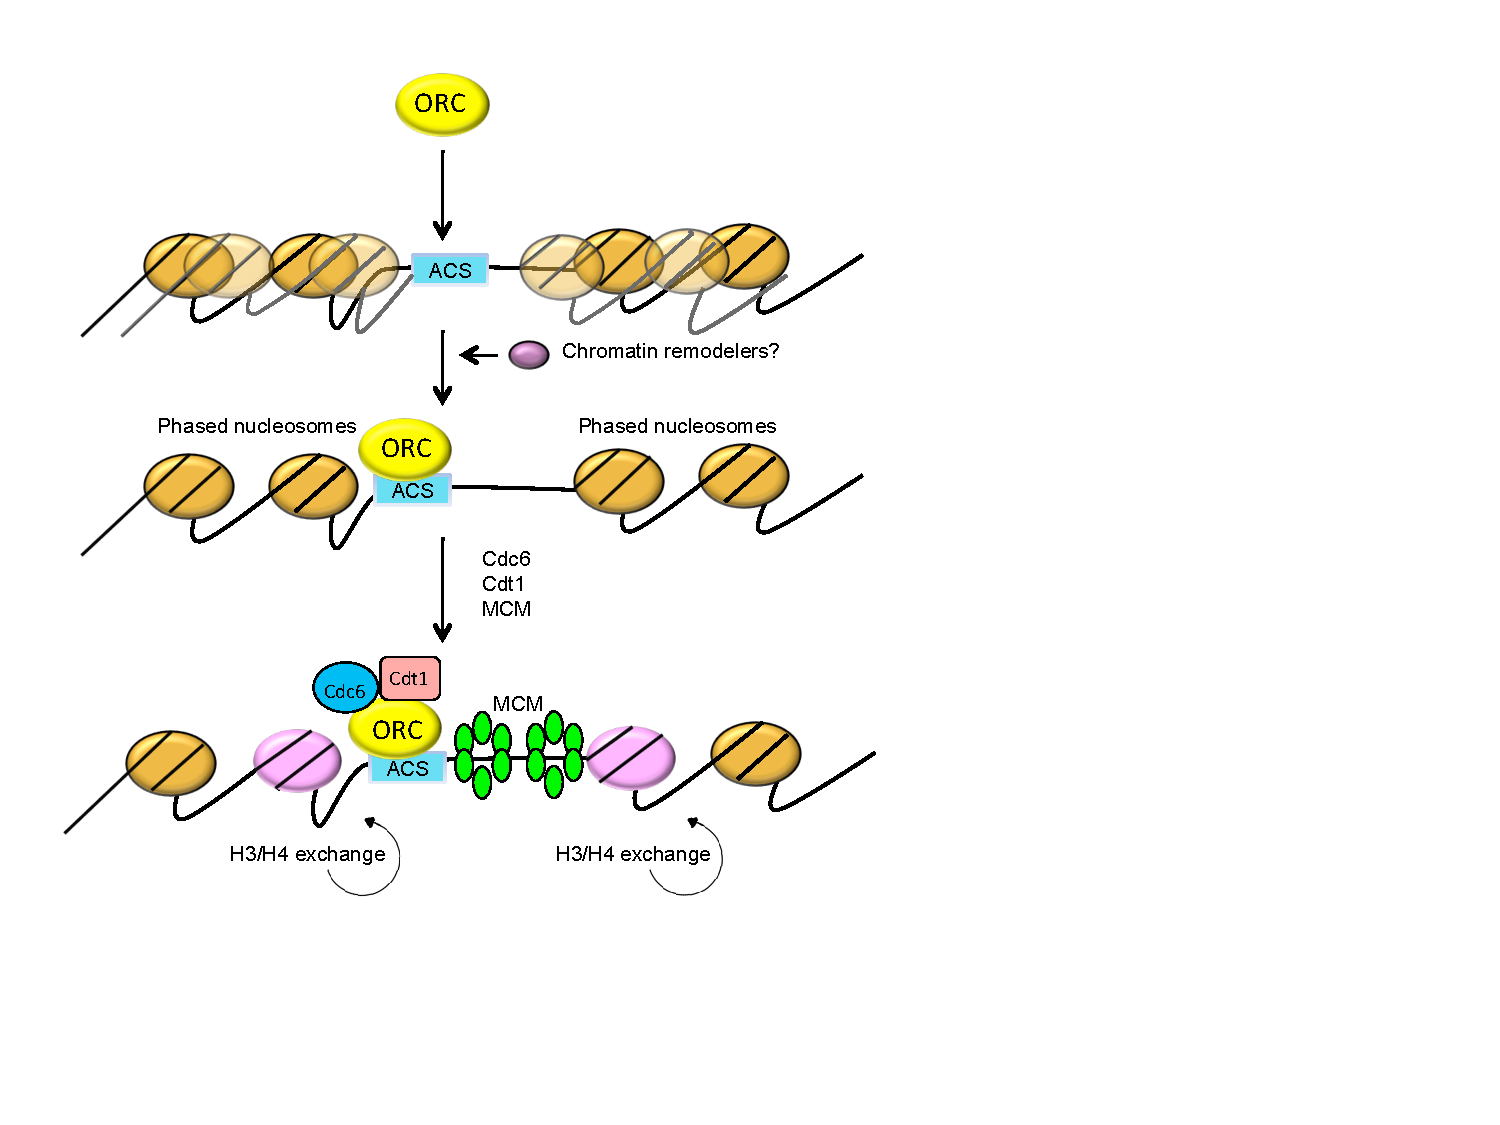
\includegraphics[width=2.5in]{r35_figures/orc_turnover_model.pdf}
%\end{center}
%\vspace{3mm}
%\caption{Pre-RC assembly at replication origins in the context of chromatin. The Mcm2-7 complex is loaded onto origins by ORC, Cdc6 and Cdt1. Nucleosome positioning and chromatin remodeling are conserved features of the eukaryotic DNA replication program\citep{Ding2011-ni}.}%
%\end{floatingfigure}

%In order to duplicate a eukaryotic chromosome within the confines of S-phase, DNA replication must begin at multiple sites along the chromosome.  Failure to completely replicate the chromosomes may result in catastrophic genomic instability\citep{Green2010-ht}.  Origins of DNA replication are defined by conserved trans-acting factors that assemble on the DNA in  a cell cycle regulated manner ({\color{dukeblue}\textbf{Figure 1}}). The origin recognition complex (ORC) functions together with Cdc6 and Cdt1 to load the Mcm2-7 helicase as a double hexamer and form the pre-replicative complex (pre-RC)\citep{Bell2013-pk}. Pre-RC assembly is limited to G1 and serves to `license' the origin for activation in the subsequent S-phase\citep{Siddiqui2013-jz}. As cells enter S-phase, DDK and CDK promote the recruitment of additional proteins to the origin including Cdc45 and the GINS complex to form the pre-initation complex (pre-IC)\citep{Tanaka2013-fl} ultimately resulting in an active helicase complex at each fork.   



%In yeast, DNA replication origins are defined by cis-acting sequence elements that are necessary, but not sufficient, for ORC binding and origin function\citep{Breier2004-tw} suggesting that additional chromatin features modulate origin selection and activation.  In higher eukaryotes ORC exhibits little sequence specificity\citep{Vashee2003-xr} and is preferentially enriched in open and accessible chromatin\citep{MacAlpine2010-ju,Miotto2016-jt}.   We and others have shown that precise nucleosome positioning and active histone exchange are conserved features of ORC binding in yeast\citep{Eaton2010-fq,Berbenetz2010-hh}, \dros\citep{Liu2015-nr,MacAlpine2010-wz} and mammalian cells\citep{Lombrana2013-aw,Lubelsky2011-dj}.  Despite the identification of specific ORC binding sites in higher eukaryotes\citep{Miotto2016-jt}, the mapping of origins has been challenging and controversial\citep{Prioleau2016-bj}.  Recent Okazaki fragment mapping across the human genome identified fewer than a dozen sites were the initiation event could be mapped within 5 kb; instead the vast majority of initiation events mapped to broad zones of 30 kb or more\citep{Petryk2016-rr}.  If ORC localizes to discrete sites of open chromatin marked by DNase I hypersenstivity\citep{MacAlpine2010-ju,Miotto2016-jt}, why are initiation events so dispersed?  One intriguing possibility is that the Mcm2-7 complex may not be restricted to ORC proximal sequences following pre-RC assembly and that the location and density of Mcm2-7 complexes on the chromatin may be responsible for the seemingly stochastic origin activation patterns observed in higher eukaryotes. Alternatively, provocative experiments from the Dutta laboratory  suggest an ORC-independent mode of Mcm2-7 loading in mammalian cancer cells\citep{Shibata2016-uc}. 


%For more than three decades the identification of specific start sites of DNA replication has been a challenge in higher eukaryotes.  Despite the advent of multiple genome-wide approaches for mapping origins, there has only been minimal concordance between different experimental assays including nascent strand abundance assays, ChIP-seq of initiation factors, and mapping replication initiation bubbles.  While some of the disagreement may be due to technical problems, it is becoming increasingly clear that origin selection and activation is a stochastic process in higher eukaryotes.  Recent studies mapping the distribution of Okazaki fragments throughout the genome found fewer than a dozen sites where robust initiation occurred within a 5 kb window, instead the majority of  initiation events mapped to large zones of 30 kb. If ORC localizes to discrete sites of DNase I hypersensitive open chromatin, how and why are the initiation zones so broad?   Recent in vitro work from the Remus lab in \scer demonstrate that the Mcm2-7 complex is able to translocate on the DNA and be pushed away from the site of loading by active transcription.  Experiments from our own laboratory have also demonstrated that active transcription can shape the genomic distribution of the Mcm2-7 complex in \dros.  Thus, a model is emerging whereby ORC loads the helicase complex at ORC binding sites, but that the Mcm2-7 complex is not fixed and is able to translocate along the chromosome.  Alternatively, provocative experiments from the Dutta laboratory may suggest an ORC-independent mode of Mcm2-7 loading in mammalian cancer cells. 

%DNA replication is also the major source of double strand breaks (DSBs) which can occur when the fork encounters nicked DNA or the collapse of a stalled replication fork\citep{Munoz2017-mi}.
%\cite{Halazonetis2008,Hanahan2000,Hanahan2010,Vignard2013}.  
%If not promptly repaired, DSBs may lead to cell death and/or complex chromosomal re-arrangements due to untethered DNA ends\cite{Morgan1998,Hinnen1978}.  
%The factors that mediate DSB recognition and repair via either homologous recombination or non-homologous end joining are molecularly and biochemically well characterized\cite{Symington2011}.
%\cite{Rogakou1999,Vignard2013,Lee2005,Lee2007,Tsukuda2005,Foster2005,Liang2007,Symington2011,Lee2014,Harrison2006,Iacovoni2010,Chai2005,Chai2005a,Burma2001,Burma2001a,Kwon2015,Kwon2014,Geuting2013,Berkovich2007,Sonoda1998,Goldstein2013,Wolner2003,Nakada2003,Shroff2004,Hicks2011,Madabhushi2015,Tsabar2016,Mehta2017,Moore2007,Krogh2004,Kim2007,Alexeev2003,Keogh2006,Costanzo2004,Kurz2004,Haber2016,Haber2012,Avsaroglu2016,Nasmyth1993,Torres-Machorro2015,Celeste2003,Lee2004,Downs2000,Shechter2004,Clapier2009,Morillo-Huesca2010,Lisby2004,Morrison2004,Kimura2006a,Kimura2006,Rothstein1991,Halazonetis2008,Sogo2002,Sugawara2003,Frank-Vaillant2002,Stracker2004,Ataian2006}.
%While nucleosome remodeling and eviction must occur at the break to facilitate strand end-resectioning and Rad51 nucleoprotein filament formation\cite{Renkawitz2014}, it is unclear how the local chromatin architecture at diverse locations throughout the genome impacts the kinetics of DSB induction, recognition and repair.
%\cite{Tsabar2016,Tsukuda2005,Jasin2013}.  

%Finally, a consequence of DNA replication is that chromatin is disassembled ahead of the replication fork; thus, the chromatin, or epigenetic state, needs to be re-established every cell division on the newly synthesized DNA\citep{MacAlpine2013-ds}.   The biochemical mechanisms of chromatin assembly at the replication fork have been well studied \invitro. However, considerably less is known about \invivo kinetics of chromatin assembly, including the association of specific transcription factors and re-establishment of nucleosome positioning behind the replication fork.  



%Stalled DNA replication forks may lead to double strand breaks (DSBs) 
%The local chromat

%F31
%Elegant genetic and biochemical experiments have elucidated many of the molecular events associated with the recognition and repair of  double strand breaks.  In addition to the factors required for break recognition, processing and repair via homologous recombination or non-homologous end joining, the local chromatin environment also influences the accessibility of the break site and the kinetics recognition and repair.  Further there are also global changes in epigenetic state and nuclear architecture that occur in a cell burdened with DSBs.   Prior experiments have identified loss of nucleosome occupancy and [specific remodeling? events] at the MAT locus; however, they have lacked the temporal and spatial resolution to discern the mechansim by which which nucleosome occupancy is lost (eg. eviction or sliding?).   In addition, it is unclear how dependent the observed changes in nucleosome occupancy are on the local chromatin structure and state of the MAT locus. 


%This model may also address provactive experiments from the Dutta laboratory suggesting that ORC is not essential for replication in mammalian cancer cells.  Either there are indpendent Mcm2-7 loading mechnanisms, or that there is some minimal ORC in the mutants (estimated to be less than 1\%) capacity that is sufficient for loading the Mcm2-7 complex. 

%image of stochastic origin selection. -- where am i going with this.

%Until recently, origin selection was thought to be dependent on ORC binding.  However, 

%Although we have begun to elucidate the chromatin determinants of o

%In addition to conserved trans-acting factors, origins of DNA replication are also defined by cis-acting sequences and  chromatin features.  In \scer, a degenerate T-rich sequence, termed the ACS (ars consensus sequence) is necessary, but not sufficient for ORC binding and origin function. However, in higher eukaryotes, ORC exhibits little sequence specificity and is preferentially enriched in open and accessible chromatin \cite{macalpine,struhl}. 

 


%with active and repressive chromatin states contributing to

%-- not surpring regulated origin activity. [also cite oscar]

%correlations individual origins

%finally -- chromatin assembly


%Chromatin faciltates the packaging and compaction of the genome and

%how to get back to replication. 

%Origin selection is not a stochastic process -- 

%Origin selection and activation are shaped by the chromatin environment and nuclear architecture.  

%In addition to conserved trans-acting factors, origins of DNA replication are also defined by cis-acting sequences and epigenetic features.  


%Overview figure
 %   nucleosome dynamics origin activation
  %  chromatin assemblyOr
   % mcm redistribution and origin activation
    %transcription
    %DNA breaks
    


%In contrast, the cis-acting sequence elements that contribute to origin function are less understood.  In \scer\ , the ACS (ARS consensus sequence) is a degenerate T-rich sequence that is necessary, but not sufficient, for ORC binding and origin function\citep{BCC04}. In addition, other poorly defined sequence elements (termed B-elements) also contribute to origin function\citep{Marahrens:1992zr}. However, in metazoan systems, ORC exhibits little if any sequence specificity \invitro\citep{VCL+03,RBB04}, suggesting that other chromosomal features (e.g. chromatin accessibility, histone modifications, transcription factors, etc) may participate in origin selection. Indeed, we and others have shown that nucleosome organization and active histone exchange are conserved features of ORC localization in \scer\citep{EGK+10} and \dros\citep{MGP+10,modENCODE-Consortium:2010vn,Eaton:2011ys}.  

%Our research program is focused on understanding how the local chromatin environment impacts the DNA replication program to maintain both genetic and epigenetic inheritance. 

%Atouble hexamer of the Mcm2-7 complex is loaded.  

%notes for donald
%Letters of Support:  The application must include a letter from the institution’s Authorized Organizational Representative (AOR) indicating that they are aware of and accept the condition that other NIGMS research awards must be relinquished and pending NIGMS research applications, except as allowed in Section I, withdrawn as a condition of receiving a MIRA, and providing a statement that if chosen to receive an award, the PD/PI will devote at least 51% of his/her time available for research to this award. The time available for research should be determined in person-months and should not include time expended toward teaching, administration, and/or clinical duties.

%cost share of 26%

%begin to assemble on the DNA in G1 of the cell cycle.

%In addition to conserved trans-acting factors, origins of DNA replication are also defined by cis-acting sequences and epigenetic features.  

%need to mention dutta paper
%hyrien paper and 


%The trans-acting factors taht


%DNA replication  assays 

%DNA replication --> huge progress
%chromatin and origin selection regulation larger view nuclear and chromatin.  We
%yeast vs rest of eukaryotic systems
%chromatin assembly
%Transcription
%DNA Damage




%Genetic and epigenetic inheritance

%Figure


%It is essential that the genome be replicated accurately and completely within the confines of S-phase. Failure to completely replicate the chromosomes may result in catastrophic genomic instability\citep{GFL10}. Replication initiates from multiple sites, termed origins of replication, along each chromosome. In metazoans, DNA replication is a dynamic process capable of responding to changes in the developmental program\citep{HMM95}. Increasing evidence suggests that the DNA replication program is regulated, in part, by the organization and accessibility of the local chromatin environment\citep{Berbenetz:2010vn,EGK+10,DHH10}. Currently, very little is known about how the architecture and dynamics of the local chromatin environment modulate the DNA replication program to maintain genomic stability.


%In all eukaryotes origin selection is mediated by the formation of a multi-protein complex, called the pre-replicative complex (pre-RC), on DNA during G1 of the cell cycle\citep{BD02}({\bf \color{dukeblue}Figure 1}). Potential origins of replication are marked by the origin recognition complex (ORC). ORC together with Cdc6p and Cdt1p cooperate to load the Mcm2-7 helicase forming the pre-RC in G1\citep{MLB06,BS08}. The pre-RC functions as an essential initiator complex, and its components are conserved in all eukaryotes. The formation of the pre-RC in G1 on the DNA in effect licenses that sequence to function as an origin of replication during the subsequent S-phase\citep{Dif04}.

%In contrast, the cis-acting sequence elements that contribute to origin function are less understood.  In \scer\ , the ACS (ARS consensus sequence) is a degenerate T-rich sequence that is necessary, but not sufficient, for ORC binding and origin function\citep{BCC04}. In addition, other poorly defined sequence elements (termed B-elements) also contribute to origin function\citep{Marahrens:1992zr}. However, in metazoan systems, ORC exhibits little if any sequence specificity \invitro\citep{VCL+03,RBB04}, suggesting that other chromosomal features (e.g. chromatin accessibility, histone modifications, transcription factors, etc) may participate in origin selection. Indeed, we and others have shown that nucleosome organization and active histone exchange are conserved features of ORC localization in \scer\citep{EGK+10} and \dros\citep{MGP+10,modENCODE-Consortium:2010vn,Eaton:2011ys}.  Our research program is focused on understanding how the local chromatin environment impacts the DNA replication program to maintain both genetic and epigenetic inheritance.  

%A mechanistic understanding of how origins are established and regulated in proliferative cells will have far-ranging implications for developmental, stem cell, and cancer biology. Failure to completely duplicate the genome {\em exactly} once per cell cycle in mitotic cells results in genomic instability\citep{GFL10} -- a hallmark of cancer. Two pre-RC components, Cdc6p\citep{GKD+06} and Cdt1p\citep{AFS+02}, have oncogenic potential, presumably mediated by re-replication induced genomic instability which can include gene amplification\citep{GFL10}. Conversely, a decrease in replication initiation (as in the {\em MCM4} ({\em chaos3}) mutant in mouse) also leads to chromosomal breaks, genome instability and cancer\citep{SAL+07}. Finally, recent studies have linked mutations in multiple components of the pre-RC (including ORC) to Meier-Gorlin syndrome, an autosomal recessive form ofdwarfism\citep{Bicknell:2011ys,Bicknell:2011zr}. Only by identifying and characterizing the specific chromosomal elements that direct and regulate DNA replication will we be able to understand how these processes are established and maintained to preserve the expression and inheritance of genetic information. 